\documentclass[letterpaper,12pt]{article}
\usepackage[top=1in, left=1.25in, right=1.25in, bottom=1in]{geometry}
\usepackage[utf8]{inputenc}
\usepackage[T1]{fontenc}
\usepackage[spanish]{babel}
\usepackage{graphicx}
\usepackage{caption}
\usepackage{float}
\usepackage[backend=biber,style=numeric,sorting=none]{biblatex}
\usepackage{amsmath}
\addbibresource{bib/referencias.bib}
\usepackage{subcaption}

\begin{document}

\tableofcontents
\clearpage

\section{Introducción}

\begin{itemize}
\item \textbf{Planteamiento del Problema:} Se busca implementar una aplicación en Java que permita representar distintas figuras geométricas, utilizando los principios de herencia y polimorfismo. La práctica consiste en crear una clase abstracta 'Figura' que defina las características y comportamientos generales, y clases derivadas que sobrescriban los métodos necesarios para calcular las áreas o perímetros, demostrando así el uso del polimorfismo en tiempo de ejecución.

\item \textbf{Motivación:} 
En esta práctica aprenderemos a utilizar la herencia para reutilizar código y establecer jerarquía entre clases, así como aprender a aplicar el polimorfismo para modificar comportamientos de manera dinámica según el tipo de objeto. 

\item \textbf{Objetivos:} 
Implementar un programa que utilice una clase abstracta y varias clases derivadas de ella para representar figuras geométricas aplicando herencia y polimorfismo. Comprender cómo las clases derivadas pueden sobrescribir métodos de la clase padre y cómo el uso de referencias polimórficas permite invocar diferentes comportamientos con una misma interfaz.


\end{itemize}
\section{Marco Teórico}
    \begin{itemize}
        \item \textbf{Herencia: }Es un concepto que permite definir nuevas clases basadas en clases ya existentes, aprovechando y extendiendo su funcionalidad, ahorrando tiempo y esfuerzo, creando una clase en base a otra con el uso de la palabra reservada 'extends' al declarar la clase.
        Se puede obtener herencia de dos tipos de clases: clases normales, lo que permite acceder a sus métodos; clases abstractas, lo que hace que la clase que heredó, solo tenga una guía de que métodos debe tener y completar.~\cite{HerenciaPolimorfismo}
        \item \textbf{Polimorfismo: }Es la capacidad de un objeto para adquirir diferentes comportamientos, mas especificamente, es el concepto de implementar métodos con el mismo nombre pero distinto comportamiento en distintas clases.~\cite{HerenciaPolimorfismo}
        \item \textbf{Clases abstractas: }Son un tipo de clases de las cuales no se puede crear un objeto a partir de ellas, pero sirven para  definir una especie de 'esqueleto' que otras clases deben seguir al momento de heredar de la clase; una clase abstracta puede contener métodos abstractos, que indican que se deben implementar en la clase que herede o metodos con comportamiento ya definido; la forma en la que se crea una clase abstracta es usando la palabra reservada 'abstract' en vez de public al momento de crear la clase.~\cite{Abstracto}
    \end{itemize}

\section{Desarrollo}
\textbf{Librerías, clases, paso de mensajes y empaquetado de clases:}
Para esta práctica se ha implementado un graficador de diferentes figuras geométricas con interfaz gráfica de usuario (GUI). Para ello, las principales librerías que se han utilizados son: 
\begin{enumerate}
    \item \textbf{javax.swing.*} : En este paquete se incluyen las clases necesarias para crear una interfaz gráfica de usuario, permite además crear ventanas, botones, listas y campos de texto.
    \item \textbf{java.awt.*} : Proporcionan clases para modificar el diseño de las ventanas (dimensiones, colores, etc).
\end{enumerate}
Todas las clases han sido organizadas o empaquetadas dentro de la carpeta: 

\textbf{/mx/unam/fi/poo/p78/}, al agregar: \textbf{package mx.unam.fi.poo.p78;} al inicio de cada clase.\\

La clase abstracta \textbf{Figura} representa un objeto genérico dentro de las figuras que se pueden crear, contiene los métodos abstractos \textbf{area()}, \textbf{perimetro()} y \textbf{dibujar()}, esta última nos ayudara a crear el dibujo de la figura seleccionada.\\

En la subclase \textbf{Circulo} heredada de \textbf{Figura}, se ha inicializado un constructor con un atributo privado llamado \textbf{radio} para el que se le han generado sus respectivos \textbf{set} y \textbf{get}. Implementamos también los métodos sobreescritos \textbf{area()}, \textbf{perimetro()} y \textbf{dibujar}.\\

Para la subclase \textbf{Rectangulo} heredada de la misma clase \textbf{Figura}, inicializamos el constructor con los atributos privados \textbf{alto} y \textbf{ancho}, con sus respectivos \textbf{setters y getters}. Igualmente incluye los métodos sobreescritos \textbf{area()}, \textbf{perimetro()} y \textbf{dibujar}.\\

Por último desarrollamos la subclase \textbf{TrianguloRectangulo} heredada de \textbf{Figura}, con su constructor, atributos privados \textbf{base} y \textbf{altura}. Nuevamente esta subclase presenta los métodos \textbf{area()}, \textbf{perimetro()} y \textbf{dibujar}.\\

 Finalmente para \textbf{MainApp} se inicializaron diversos atributos, que sirven para crear la ventana (frame), lista desplegable para crear figuras (comboFiguras), pies de página para los campos de texto (l1, l2), campos de texto(t1, t2), muestra del área y perímetro calculados (areaLbl, perLbl), panel donde se dibuja la figura (panelDibujo) y cadenas de texto fijas para identificar a las figuras(FIGCIRCULO, FIGRECTANGULO, FIGTRIANGULO).\\
 Los métodos implementados son: 
 \begin{enumerate}
     \item \textbf{crearGUI()}: Crea la ventana principal de la aplicación.
     \item \textbf{actualizarFormulario()}: Sirve para actualizar las etiquetas (l1, l2), los campos (t1, t2) y el estado de la interfaz según la figura seleccionada. 
     \item \textbf{calcularYDibujar()}: Lee los valores numéricos, crea el objeto de la figura, calcula su área y perímetro, y lo manda a dibujar.
     \item \textbf{main()}: Inicia la interfaz gráfica
 \end{enumerate}
 
\clearpage

\section{Resultados}

\begin{figure}[H]
    \centering
    \begin{subfigure}{0.6\textwidth}
        \centering
        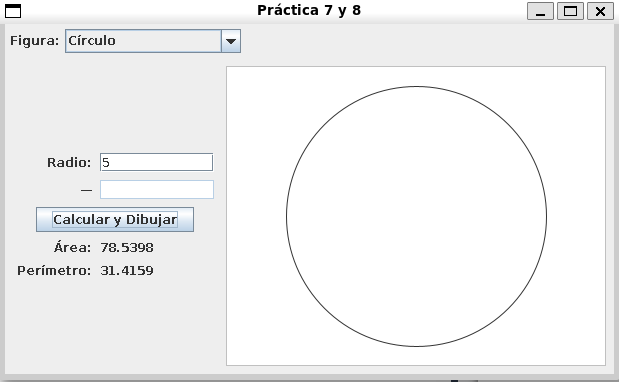
\includegraphics[width=\linewidth]{Imagenes/circulo.png}
        \caption*{Pruebas de circulo}
    \end{subfigure}
    \hfill
    \begin{subfigure}{0.6\textwidth}
        \centering
        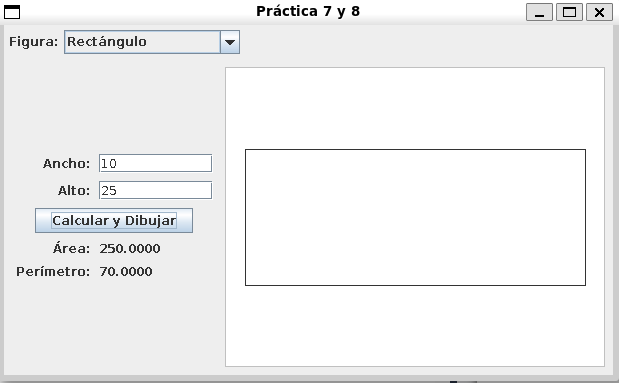
\includegraphics[width=\linewidth]{Imagenes/rectangulo.png}
        \caption*{Pruebas de rectángulo}
    \end{subfigure}
    \hfill
    \begin{subfigure}{0.6\textwidth}
        \centering
        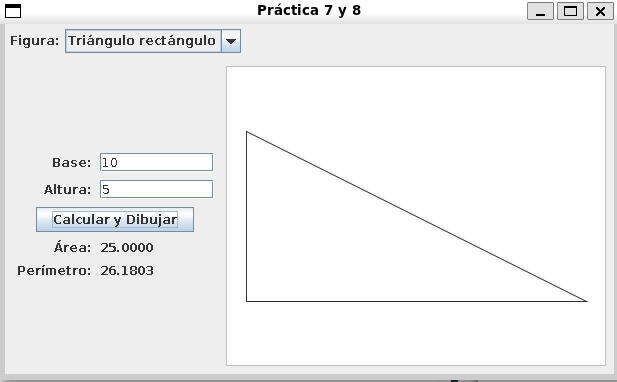
\includegraphics[width=\linewidth]{Imagenes/triangulo.png}
        \caption*{Pruebas de triangulo}
    \end{subfigure}
\end{figure}

\clearpage

\section{Conclusiones}

La práctica nos permitió comprender y aplicar de manera efectiva los conceptos de herencia y polimorfismo en Java, observando cómo es que una clase abstracta puede servirnos como una base para definir comportamientos generales que las clases derivadas adaptan según sus necesidades. A través de la creación de distintas figuras geométricas, se demostró cómo el polimorfismo en tiempo de ejecución posibilita invocar métodos sobrescritos de forma dinámica, facilitando la extensibilidad y reutilización del código. En conjunto, la práctica nos permitió fortalecer la comprensión de la programación orientada a objetos, destacando la importancia de diseñar jerarquías de clases bien estructuradas para lograr programas más flexibles, organizados y eficientes.

\printbibliography

\clearpage

\section{Reto para token}

Para el desarrollo de este token, realizamos la implementación de la clase 'Material', que es la clase padre de las clases 'Revista', 'DVD' y 'Libro'. Cada clase sobrescribe un método llamado 'mostrarInformacion', que se sobrescribe para cada material y se utiliza para imprimir su información correspondiente

Dentro del 'main', creamos un menú donde se le da a elegir al usuario que tipo de material quiere agregar, y mediante polimorfismo se convierte un objeto de tipo 'Material' en el seleccionado por el usuario. Cada material es guardad en un 'ArrayList' utilizado para imprimir los materiales ingresados.

\begin{figure}[H]
    \centering
    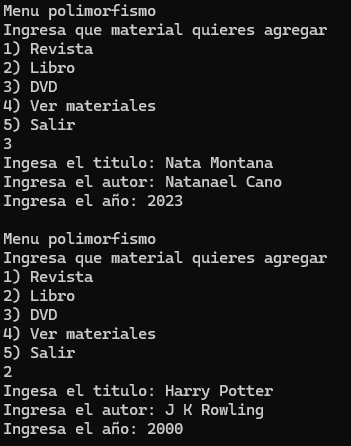
\includegraphics[width=0.45\linewidth]{Imagenes/a.png}
    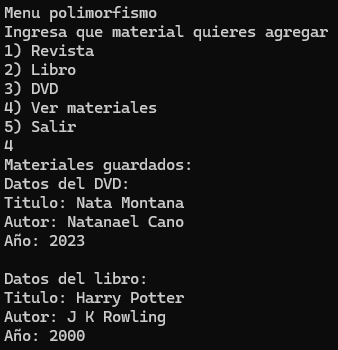
\includegraphics[width=0.45\linewidth]{Imagenes/s.png}
    \caption*{Ejecución}
\end{figure}

\end{document}